
Grid computing \cite{li2005grid} is the most recent decade's technology
innovation in high performance computing. A large number of scientistcs working
on the operations of this huge co-operative project of EU. Monitoring \&
information architecture \cite{fisher2002datagrid} has been standardized in the
initial state of that project, to succeed in today scale of 150.000 cores. Use
of grid computing nowadays takes place in academic and research environments,
but applications in industry-based needs such as promising Power Grid control
\cite{Taylor2006} are emerging.

\section{Grid Monitoring}
Standards are being published about the operational models that the grid
computing initiative will use. Last decade the EGEE I, II \& III was adopted by
european universities to fund and establish a collaborative community of
researchers under a central point, the CERN oriented research project in
Particle Physics. After EGEE, the European Grid Initiative were formed to lead
to the explode of that community into regional initiatives. Performance
and availability monitoring tools and views also follow that format, phasing out
commonly used SAM \cite{egee3dsa122} and having the adoption of Nagios as the
monitoring of regional performance tool.

\section{Resource Brokers}
Resource Brokers \cite{Kertesz06ataxonomy} where developed to manage the
workload on Computer elements and Resource elements. Globus which is 
non-service based RB was replaced by gLite RB which is service based. A Workload
Management System (WMS) exists in gLite to do the distribution and management of
the Computing and Storage oriented tasks.

% TODO here may reside the image of taxonomy of resource brokers based on the IS

\subsection{Globus}
\subsection{gLite}

% TODO to gLite monitoring me dika mou logia
The ability to monitor resource related parameters is currently considered a
necessary functionality in any network. In such a heterogeneous and complex
system as the Grid, this necessity becomes fundamental. A monitoring system
implies the existence of a central repository of operational information (in
WLCG/EGEE, the GOCDB). The monitoring system should be able to collect data from
the resources in the system, in order to analyze the usage, behavior and
performance of the Grid, detect and notify fault conditions, contract violations
and user-defined events.
The GOC web page contains a whole section
concerning monitoring information for WLCG/EGEE. Several different monitoring
tools are in use, including general-purpose monitoring tools and Grid specific
systems.
Also important are the web pages publishing the results of functional tests
applied periodically using the Service Availability Monitoring (SAM) to the all
the sites registered within WLCG/EGEE. The results of these tests show if a site
is responding correctly to standard Grid operations; otherwise, an investigation
on the cause of the unexpected results is undertaken. Some VOs may even decide
to automatically exclude from their BDII the sites that are not passing the
functional tests successfully, so that they do not appear in the IS and are not
considered for possible use by their applications.
%%
% https://edms.cern.ch/file/722398/1.3/gLite-3-UserGuide.html#SECTION00073000000000000000



\section{Architecture}
A Grid Monitoring Architecture \cite{tierney2002grid} was proposed in early
2000's. Information systems were developed to create repositories of information
needed to be stored for monitoring and statistical reporting reasons. Such an
organized system later was specified by the Aggregated Topology Provider (ATP)
definition. The largest world grids adopt that model, forming OIM in OSG (USA)
and GOCDB as that information base in EGEE (Europe). Message Bus was also
defined as a mean to tranfer the undelying data, and well known tools came up
such as Gstat, GOCDB and BDII with Glue specification. Grid performance
monitoring and keeping of such an information system has also impact in the
performance of the system itshelf \cite{zhang2003performance}, so various
methods were developed to give the solution to the scalling and performance
problem, such as MDS2 (GIIS \& GRIS), GMA and R-GMA
\cite{wilson2004information}, which offers relational environment
\cite{fisher2001relational}, has experience on production systems 
\cite{byrom-production} and scales to reach huge needs such as CMS project
\cite{Bonacorsi2004,Byrom}.


\begin{figure}[htb]
\centering
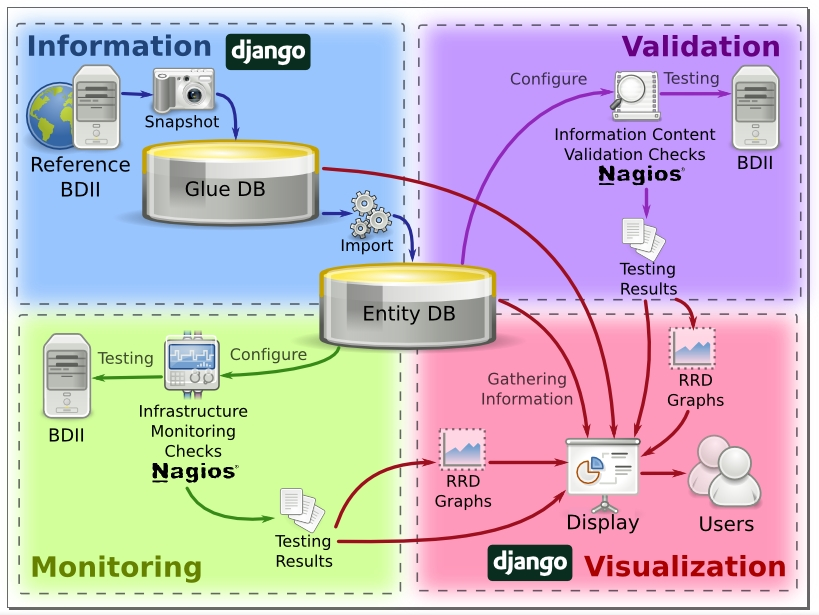
\includegraphics[width=150mm]{images/gstat-architecture.jpg}
\caption{Gstat Architecture}
\label{figure:gstat-arch}
\end{figure}

\subsection{MDS}
\subsubsection{History}

\subsection{XML based schemata}
\subsubsection{GRAM}
\subsubsection{Crux}

\subsection{Glue}
Open Grid Forum, GLUE Working Group \& GLUE specification v. 2.0
LDAP Schema Implementation (draft) \& recommended LDAP DIT

\url{http://forge.gridforum.org/sf/go/doc15518?nav=1}

CE \& SE elements in schema
Performance monitoring attributes

Schema developed by DataTAGfor EU/USA interoperability


\begin{figure}[htb]
\centering
 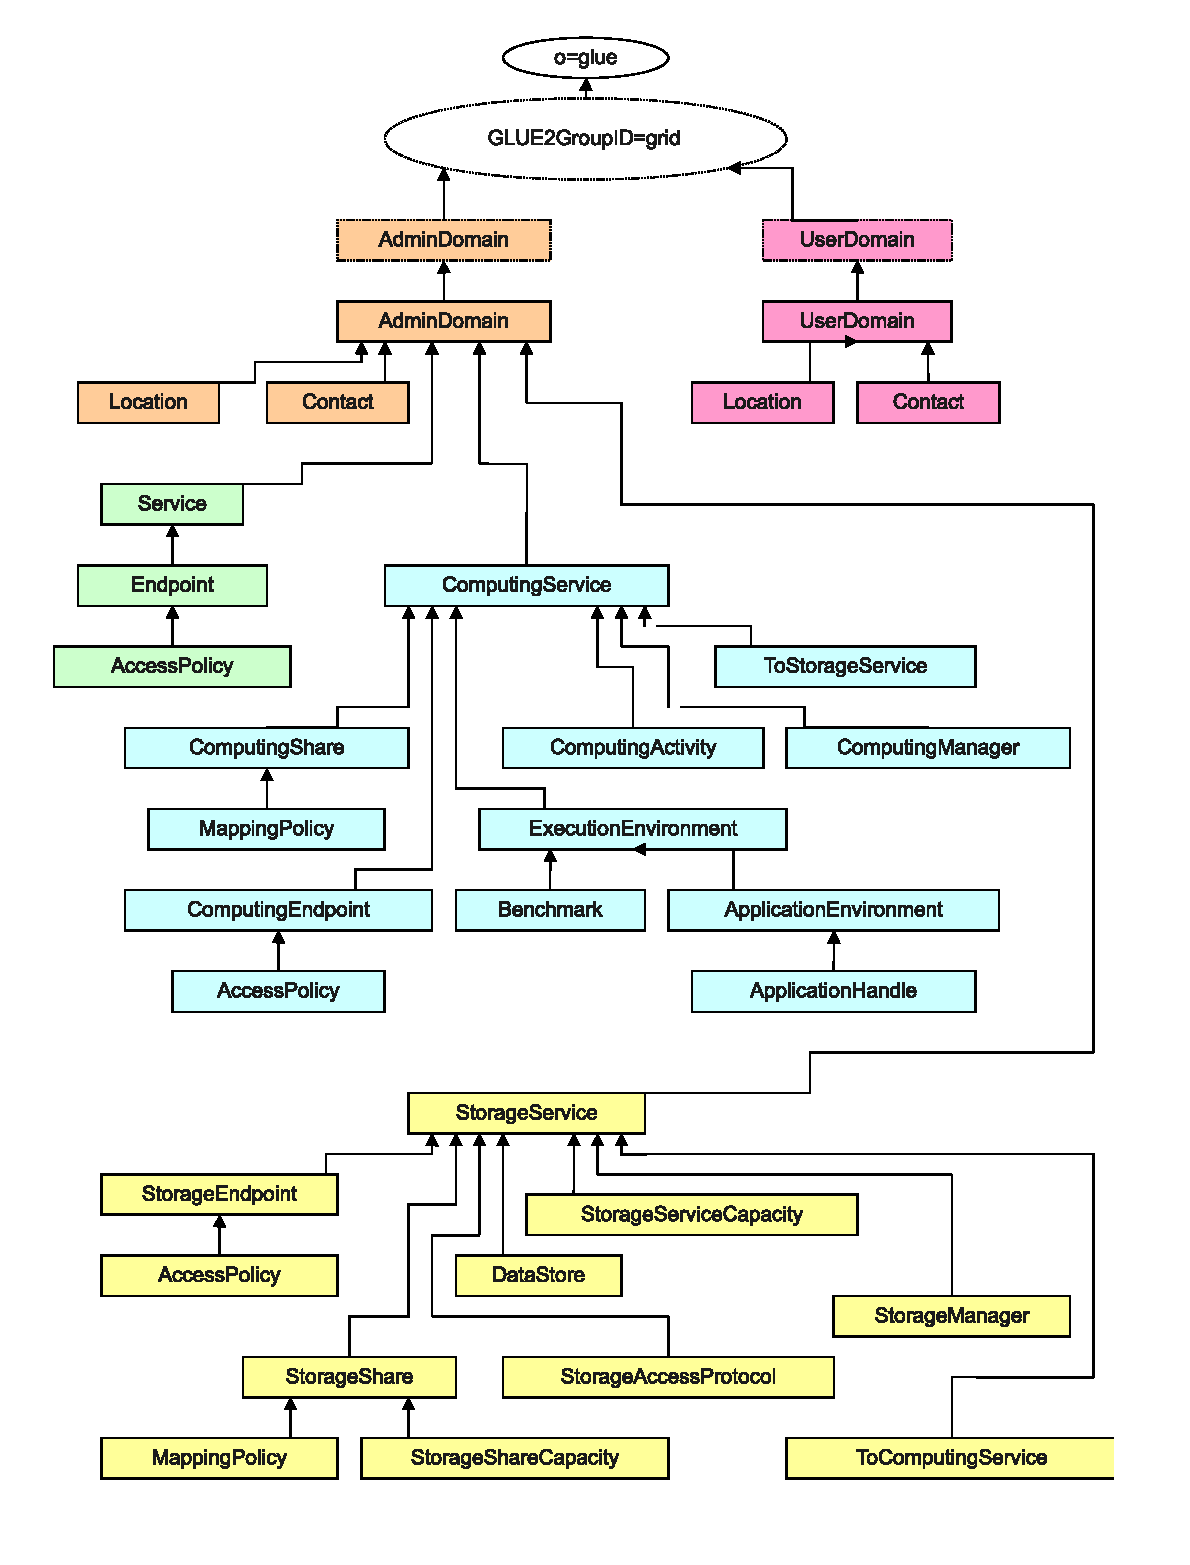
\includegraphics[width=6in]{images/glue2}
\caption{LDAP DIT}
\label{figure:gluedit}
\end{figure}

\subsection{BDII}




\section{monitoring framework}

\subsection{ATP}
Aggregated Topology Provider (ATP) : ATP is a repository of grid topology
containing information about projects (WLCG), grid infrastructures (EGEE, OSG,
NDGF), Sites, Services, VOs and their groupings, site / service downtimes and
its history. It synchronizes topology information from OSG IM, GOCDB and BDII.

\subsection{MDDB}
Metric Description Database (MDDB) : Project-level component that contains
meta-data about metrics and how those metrics can be combined to calculate
different availabilities.

\subsection{MRS}
Metric Result Store (MRS) : A Repository of metric results containing Metric
results for service end-points for the grid infrastructure.

\subsection{ACE}
Availability Computation Engine (ACE) : The Availability Computation Engine
(ACE) module computes availability of Grid Resources using Test Results form
MRS, topology data from ATP and profile definition from MDDB. It supports
multiple algorithms for computation of Grid Resources.


\section{Tools}
A taxonomy effort has been made \cite{gerndt2004performance} to present the
differencies of performance monitoring systems of the grid, and later a more
general \cite{zanikolas2007importance} taxonomy paper was published to give a
more general visibility of these tools. GridICE was generaly used to aggregate
the performance metrics of ROCs in high level reports
\cite{andreozzi2005gridice}. Later GridICE was left as long as the SAM left, to
meet the milestone of EGI to have a regional monitoring tool (Nagios) to report
the reliability of the joined sites and report the values for SLA reasons.

\section{Sam to Nagios}
Latest EGI directive to form regional operation tools pushed the use of Nagios
\cite{imamagic2007grid} as the main tools of availability \& performance (an so
reliability) monitoring of the grid. Each NGI/ROC (regional level) has its own
interface, and hierarhicaly there is a Super Nagios interface to report the top
level view of general system availability. Nagios offers extensions such as NRPE
to remotely invoke check commands in inaccesible/private installations.
Another important add-on to Nagios is the NdoUtils, which offers an SQL store
of history data to the monitoring interface. Nagios Configuration Generator was
introduced to help the automaticaly generation of the configuration based on
the information system of nodes and services. Finally, there has been proposed
an integration of SAM views to a Nagios customized interface, to offer the last
good known SAM interface to the old users. Nagios also integrates with GGUS, a
ticketing system that european grid initiative uses.


\section{NGS}
Brunel Univesity takes part in regional and european initiatives. 4 different
Computer Elements exist, and 3 Storage Elements, consisting the UKI-LT2-Brunel
site. LT2 stands for London Grid, a co-operation with other London Universities.
GridPP and NGS are two collaboration groups that Brunel Univesity is member of,
and papers on the web interface \cite{Hobson2007} and real time visualization of
the grid status were presented \cite{Huang2007} by GridPP
